\chapter{الفلزات الانتقالية ومعقدات التناسق}\label{ch:b2:coordination-complexes}

في سنة 1893 شرع كيميائي في السادسة والعشرين، ألفرد فرنر، في تفسير لغز.
يكوّن كلوريد الكوبالت(III) أربعة مركبات مع الأمونيا، \ce{CoCl3.6NH3}
و\ce{CoCl3.5NH3} ومركبين صيغتهما \ce{CoCl3.4NH3}، أحدهما أخضر والآخر بنفسجي.
ويرسّب نترات الفضة الكلوريدات الثلاثة في الأول دفعة واحدة، واثنين من
الثاني، وواحدًا فقط من كل من الأخيرين. وجواب فرنر --- ست
مجموعات مثبتة حول الفلز عند رؤوس ثماني أوجه، والباقي خارجها
--- أسس كيمياء التناسق. ويوسّع هذا الفصل معقدات
مجلد السنة الأولى لتشمل هندستها، ومتماكباتها، وأسماءها، وعدًّا
للإلكترونات يتنبأ بكربونيلات الفلزات الموجودة.

\begin{recall}
مجلد السنة الأولى: المعقد، والذرة المركزية، والربيطة، والربيطة المتعددة المخالب، والمعقد المخلبي،
وثوابت التكوين، وعدد التناسق؛ والتوزيعات الإلكترونية لأيونات
الفلزات الانتقالية (تُفقد إلكترونات \babelsublr{$n$s} أولًا)؛ وأحماض لويس وقواعده،
والروابط التساندية؛ ونموذج VSEPR؛ وأعداد الأكسدة؛ والمتماكبات المرآوية. و\cref{ch:b2:atomic-orbitals}:
مدارات d وترتيب المستويين 4s و3d.
\end{recall}

\begin{omfigure}
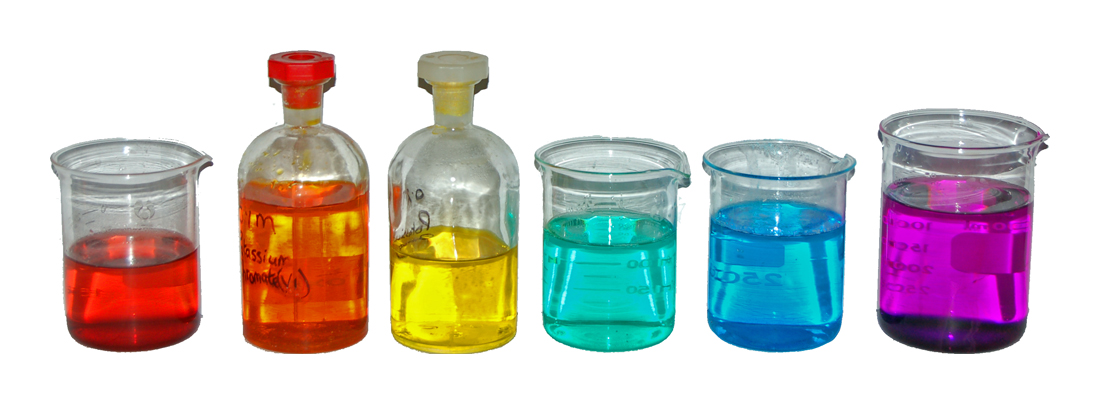
\includegraphics[width=0.8\linewidth]{images/book3/tm-solutions.jpg}

{\small محاليل مائية لمركبات فلزات انتقالية: من اليسار إلى اليمين،
نترات الكوبالت(II)، وثنائي كرومات البوتاسيوم، وكرومات البوتاسيوم، وكلوريد النيكل(II)،
وكبريتات النحاس(II) وبرمنغنات البوتاسيوم. وألوان محاليل الكوبالت والنيكل
والنحاس مصدرها معقداتها المائية. (صورة: بنجاه بي إم إم 27،
ملكية عامة، ويكيميديا كومنز.)}
\end{omfigure}

\section{الفئة d}

\begin{definition}[العنصر الانتقالي]\label{def:b2:coordination-complexes:transition-element}
\emph{العنصر الانتقالي}\index{عنصر انتقالي} عنصر لذرته، أو
لأحد أيوناته الشائعة، طبقة فرعية d ممتلئة جزئيًا. ويكون لأيون مثل هذا العنصر
فيه $n$ إلكترونًا في مداراته d \emph{توزيع $d^n$}\index{توزيع dn@توزيع $d^n$}.
\end{definition}

\begin{proposition}[عدّ إلكترونات d]\label{prop:b2:coordination-complexes:dn}
لأيون الفلز الانتقالي $\mathrm M^{m+}$ من الزمرة ذات الرقم $g$ (من 3 إلى 12) توزيع $d^n$
مع $n = g - m$.
\end{proposition}

\begin{proof}
للذرة المتعادلة $g$ إلكترونًا بعد الغاز النبيل السابق، في المدارات \babelsublr{$n$s} 
و\babelsublr{$(n - 1)$d}. وفي الأيونات، تقع مدارات d تحت المدار s
(\cref{ex:b2:atomic-orbitals:iron}): فكل إلكترونات التكافؤ الباقية، وعددها $g - m$، إلكترونات
d.
\end{proof}

مثلًا \ce{Fe^2+} (الزمرة 8) توزيعه $d^6$، و\ce{Cu^2+} (الزمرة 11) $d^9$، و\ce{Co^3+} (الزمرة 9)
$d^6$، و\ce{Pt^2+} (الزمرة 10) $d^8$.

\section{الربائط}

\begin{definition}[عدد المخالب]\label{def:b2:coordination-complexes:denticity}
\emph{عدد المخالب}\index{عدد المخالب} لربيطة هو عدد ذراتها المرتبطة
بالذرة المركزية نفسها. و\emph{الربيطة الأحادية المخلب}\index{ربيطة أحادية المخلب} ترتبط
بذرة واحدة (\ce{H2O}، \ce{NH3}، \ce{Cl-}، \ce{CO})، و\emph{الربيطة الثنائية
المخلب}\index{ربيطة ثنائية المخلب} بذرتين (الإيثان-1،2-ثنائي الأمين، ويُكتب en؛ 
وأيون الإيثانديوات، ox). و\emph{الربيطة الجسرية}\index{ربيطة جسرية} ترتبط بذرتين
فلزيتين في آن واحد. و\emph{الربيطة الثنائية الموقع}\index{ربيطة ثنائية الموقع} يمكن أن ترتبط
عبر إحدى ذرتين مختلفتين، مثل أيون النتريت (عبر N أو O) أو
الثيوسيانات (عبر S أو N).
\end{definition}

\begin{definition}[كرة التناسق]\label{def:b2:coordination-complexes:coordination-sphere}
\emph{كرة التناسق}\index{كرة التناسق} لمعقد هي مجموعة
الذرة المركزية والربائط المرتبطة بها، وتُكتب بين قوسين معقوفين؛ أما الأيونات
الواقعة خارج القوسين فأيونات مضادة، غير مرتبطة بالفلز.
\end{definition}

\begin{omfigure}
\setchemfig{atom sep=2.2em}
\chemfig{M*5(-H_2N-CH_2-CH_2-NH_2-)}
\qquad
\chemfig{M*5(-O-(=O)-(=O)-O-)}
\qquad
\chemfig{N(-[:120]CH_2COO^{-})(-[:240]CH_2COO^{-})-CH_2-CH_2-N(-[:60]CH_2COO^{-})(-[:-60]CH_2COO^{-})}

\medskip
{\small ربائط مخلبية. يمينًا: الإيثان-1،2-ثنائي الأمين (en)، ثنائي المخلب عبر ذرتي
النيتروجين. وسطًا: أيون الإيثانديوات (ox)، ثنائي المخلب عبر ذرتي أكسجين. يسارًا:
أنيون edta، الذي يلتف حول أيون فلزي بذرتي نيتروجين وأربع ذرات
أكسجين كربوكسيلاتية (سداسي المخلب).}
\end{omfigure}

\section{أعداد التناسق والهندسات}

اثنان وأربعة وستة هي أكثر أعداد التناسق شيوعًا. فالفضة(I) والذهب(I) تعطيان
معقدات خطية (\ce{[Ag(NH3)2]+})؛ وتكوّن أربع ربائط رباعي أوجه
(\ce{[CoCl4]^2-}، \ce{[Zn(NH3)4]^2+}) أو مربعًا (\ce{[PtCl4]^2-}، \ce{[Ni(CN)4]^2-})؛
وخمس، هرمًا ثنائيًا مثلثي القاعدة (\ce{Fe(CO)5})؛ وست، وهي الحالة الأكثر شيوعًا بفارق كبير،
ثماني أوجه.

\begin{omfigure}
\begin{tikzpicture}[font=\small]
  \node[omligand] at (-0.8,0) {}; \node[omligand] at (0.8,0) {};
  \draw[thick, black!70] (-0.8,0) -- (0.8,0); \node[ommetal] at (0,0) {};
  \node at (0,-1.5) {\foreignlanguage{arabic}{خطي، 2}};
  \pic at (3,0) {omtetrahedron}; \node at (3,-1.5) {\foreignlanguage{arabic}{رباعي الأوجه، 4}};
  \pic at (6,0) {omsquareplanar}; \node at (6,-1.5) {\foreignlanguage{arabic}{مربع مستوٍ، 4}};
  \pic at (9,0) {omtbp}; \node[align=center] at (9,-1.65) {\foreignlanguage{arabic}{هرم ثنائي}\\ \foreignlanguage{arabic}{مثلثي القاعدة، 5}};
  \pic at (12,0) {omoctahedron}; \node at (12,-1.5) {\foreignlanguage{arabic}{ثماني الأوجه، 6}};
\end{tikzpicture}

{\small هندسات التناسق الشائعة (الفلز برتقالي، والربائط رمادية؛ والروابط
المتقطعة تتجه إلى خلف الصفحة).}
\end{omfigure}

نموذج VSEPR، الذي يضع أزواج الإلكترونات للذرة المركزية على أبعد ما يمكن بعضها عن بعض،
يخفق هنا: فأيون $d^8$ مثل \ce{Pt^2+} يحمل أربعة أزواج من إلكترونات d وأربع
ربائط، ومع ذلك فمعقداته مربعة، لا رباعية الأوجه ولا ثمانية الأوجه. فإلكترونات
d ليست أزواجًا متمركزة تدفع الربائط: بل تتعلق طاقاتها
بالهندسة على نحو يحسبه الفصل التالي.

\begin{proposition}[المعقدات المربعة المستوية $d^8$]\label{prop:b2:coordination-complexes:square-planar}
المعقدات الرباعية التناسق لأيونات $d^8$ من السلسلتين الانتقاليتين الثانية والثالثة
(\ce{Pd^2+}، \ce{Pt^2+}، \ce{Au^3+}) مربعة مستوية.
\end{proposition}

\admitted

يأتي التفسير، أي انشطار مستويات d بفعل الربائط، في
\cref{ch:b2:ligand-field}.

\section{المتماكبات}

\begin{definition}[متماكبات المعقدات]\label{def:b2:coordination-complexes:isomers}
في معقد ثماني الأوجه $\mathrm{MA_3B_3}$، يحمل \emph{المتماكب fac}\index{متماكب fac}
الربائط B الثلاث على وجه واحد من ثماني الأوجه، و\emph{المتماكب
mer}\index{متماكب mer} على خط زوال (ثلاثة مواضع في مستوٍ يمر
بالفلز). و\emph{متماكبات الارتباط}\index{متماكبات الارتباط} تختلف بالذرة التي
ترتبط عبرها \omterm{def:b2:coordination-complexes:denticity}{ربيطة ثنائية الموقع}. و\emph{متماكبات التأين}\index{متماكبات التأين}
تتبادل ربيطة مع أيون مضاد، فتعطي أيونات مختلفة في المحلول.
\end{definition}

\begin{proposition}[عدّ متماكبات ثماني الأوجه]\label{prop:b2:coordination-complexes:isomer-count}
في ثماني الأوجه، للمعقد $\mathrm{MA_4B_2}$ متماكبان (cis وtrans)، وللمعقد $\mathrm{MA_3B_3}$ متماكبان
(fac وmer)، وللمعقد $\mathrm M(\mathrm{AA})_3$، ذي الربائط الثلاث الثنائية المخلب، متماكبان
مرآويان، $\Delta$ و$\Lambda$.
\end{proposition}

\begin{proof}
في ثماني الأوجه يكون أي موضعين إما متجاورين (cis، $90^\circ$) وإما متقابلين
(trans، $180^\circ$): ترتيبان للربيطتين B. ومن أجل ثلاث ربائط B،
فإما ألا يكون أي اثنين منها في وضع trans (فتشغل وجهًا واحدًا: fac) وإما أن يكون زوج واحد بالضبط في وضع trans (
والثالثة cis بالنسبة إلى كليهما: mer)؛ ولا توجد ثلاثة مواضع متقابلة مثنى مثنى. ومن أجل
$\mathrm M(\mathrm{AA})_3$، يمتد كل مخلب على موضعين cis؛ وتلتف المخالب الثلاثة
حول المحور الثلاثي كشفرات مروحة، دائرة إما مع عقارب الساعة
وإما عكسها حين يُنظر إليها على طول ذلك المحور: صورتان مرآويتان، غير قابلتين للتطابق
لأن المعقد بلا مستوي مرآة.
\end{proof}

\begin{omfigure}
\begin{tikzpicture}[font=\scriptsize]
  \pic (a) at (0,0) {omoctahedron};
  \node[omligand, fill=omDef!70] at (a-L1) {}; \node[omligand, fill=omDef!70] at (a-L3) {};
  \node at (0,-1.5) {\small cis-$\mathrm{MA_4B_2}$};
  \pic (b) at (3,0) {omoctahedron};
  \node[omligand, fill=omDef!70] at (b-L1) {}; \node[omligand, fill=omDef!70] at (b-L2) {};
  \node at (3,-1.5) {\small trans-$\mathrm{MA_4B_2}$};
  \pic (c) at (6.5,0) {omoctahedron};
  \node[omligand, fill=omThm!70] at (c-L1) {}; \node[omligand, fill=omThm!70] at (c-L3) {}; \node[omligand, fill=omThm!70] at (c-L5) {};
  \node at (6.5,-1.5) {\small fac-$\mathrm{MA_3B_3}$};
  \pic (d) at (9.5,0) {omoctahedron};
  \node[omligand, fill=omThm!70] at (d-L1) {}; \node[omligand, fill=omThm!70] at (d-L2) {}; \node[omligand, fill=omThm!70] at (d-L3) {};
  \node at (9.5,-1.5) {\small mer-$\mathrm{MA_3B_3}$};
\end{tikzpicture}

\medskip
\begin{tikzpicture}[font=\scriptsize]
  \foreach \xs/\s/\lab in {0/1/{$\Delta$}, 4.5/-1/{$\Lambda$}} {
    \begin{scope}[xshift=\xs cm, xscale=\s]
      \draw[black!30] (0,0) circle (1.2);
      \foreach \a in {90, 210, 330} {
        \coordinate (p) at (\a:1.1); \coordinate (q) at (\a+70:0.55);
        \draw[very thick, omDef] (\a:1.1) .. controls (\a+30:1.25) and (\a+60:0.9) .. (\a+75:0.55);
        \node[omligand] at (\a:1.1) {}; \node[omligand] at (\a+75:0.55) {};
      }
      \node[ommetal] at (0,0) {};
    \end{scope}
    \node at (\xs,-1.6) {\small \lab};
  }
  \draw[densely dashed] (2.25,-1.3) -- (2.25,1.3);
  \node[anchor=south] at (2.25,1.3) {مرآة};
\end{tikzpicture}

{\small في الأعلى: المتماكبان cis وtrans للمعقد $\mathrm{MA_4B_2}$ (الربائط B زرقاء)، والمتماكبان fac وmer
للمعقد $\mathrm{MA_3B_3}$ (B حمراء). في الأسفل: المتماكبان المرآويان لمعقد ثلاثي المخلب مثل
\ce{[Co(en)3]^3+}، منظورًا على طول المحور الثلاثي، رسم تخطيطي: كل مخلب (قوس
أزرق) يصل موضعًا علويًا بموضع سفلي، والثلاثة تدور في اتجاه ($\Delta$) أو في
الاتجاه الآخر ($\Lambda$).}
\end{omfigure}

\section{الأسماء وعدّ الإلكترونات}

\begin{method}[تسمية معقد]\label{met:b2:coordination-complexes:naming}
\begin{enumerate}
  \item في الصيغة، اكتب \omterm{def:b2:coordination-complexes:coordination-sphere}{كرة التناسق} بين قوسين معقوفين، الفلز
        أولًا، ثم الربائط؛ وشحنة المعقد خارجهما.
  \item في الاسم، اذكر الربائط بالترتيب الألفبائي مع بادئات
        التضعيف (ثنائي، ثلاثي، رباعي؛ وبيس، وتريس لأسماء الربائط المركبة): تنتهي أسماء الربائط
        الأنيونية باللاحقة «-و» (كلوريدو، سيانيدو، أوكسيدو، هيدروكسيدو)، وتحتفظ الربائط المتعادلة
        بأسمائها (أكوا، أمين، كربونيل).
  \item ثم الفلز، مع اللاحقة «-ات» إذا كان المعقد أنيونًا (حديدات،
        نحاسات، كوبالتات)، ورقم أكسدته بالأرقام الرومانية.
  \item تُسمّى الكاتيونات قبل الأنيونات: فالمركب \ce{[Co(NH3)6]Cl3} هو
        كلوريد سداسي أمين الكوبالت(III)، و\ce{K4[Fe(CN)6]} هو
        سداسي سيانيدو حديدات(II) البوتاسيوم.
\end{enumerate}
\end{method}

\begin{definition}[عدّ الإلكترونات]\label{def:b2:coordination-complexes:electron-count}
\emph{عدد إلكترونات التكافؤ}\index{عدد إلكترونات التكافؤ} لمعقد هو
عدد إلكترونات d لأيون الفلز مضافًا إليه الإلكترونات التي تقدمها الربائط (اثنان
لكل زوج مانح). وتنص \emph{قاعدة الثمانية عشر إلكترونًا}\index{قاعدة الثمانية عشر إلكترونًا} على أن
المعقدات المستقرة لفلزات منخفضة حالة الأكسدة مع ربائط قوية الارتباط مستقبِلة لإلكترونات $\pi$
مثل \ce{CO} تميل إلى أن يكون لها 18 إلكترون تكافؤ.
\end{definition}

\begin{definition}[الهابتية]\label{def:b2:coordination-complexes:hapticity}
\emph{الهابتية}\index{هابتية} لربيطة هي عدد ذراتها المرتبطة
بالفلز عبر نظام $\pi$ واحد متصل؛ وتُكتب $\eta^n$: فالإيثين المرتبط
برابطته $\pi$ هو $\eta^2$، وحلقة البنتاديينيل الحلقي المرتبطة بكربوناتها الخمسة كلها $\eta^5$.
\end{definition}

\begin{method}[عدّ الإلكترونات]\label{met:b2:coordination-complexes:electron-count}
\begin{enumerate}
  \item أسند شحنات إلى الربائط بوصفها أنواعًا ذات طبقات مغلقة (\ce{Cl-}، \ce{H-}،
        \ce{C5H5-}؛ و\ce{CO}، \ce{PR3}، \ce{NH3} متعادلة) واستنتج حالة
        أكسدة الفلز.
  \item عُدّ إلكترونات d للفلز، $n = g - m$.
  \item أضف إلكترونين لكل زوج مانح: زوج لكل \omterm{def:b2:coordination-complexes:denticity}{ربيطة أحادية المخلب}، وستة للمجموعة
        $\eta^5$-\ce{C5H5-}، وستة للبنزين $\eta^6$، واثنان للألكين $\eta^2$.
  \item تُحسب الرابطة فلز--فلز إلكترونًا واحدًا لكل فلز.
\end{enumerate}
\end{method}

\begin{proposition}[كربونيلات الفلزات]\label{prop:b2:coordination-complexes:eighteen}
للكربونيلات الثنائية المستقرة من السلسلة الانتقالية الأولى \ce{Cr(CO)6}
و\ce{Fe(CO)5} و\ce{Ni(CO)4} و\ce{Mn2(CO)10} كلها 18 إلكترون تكافؤ لكل ذرة
فلز.
\end{proposition}

\begin{proof}
الكروم(0)، $d^6$، مع ست ربائط CO: $6 + 12 = 18$. والحديد(0)، $d^8$، مع خمس CO: $8 + 10 = 18$.
والنيكل(0)، $d^{10}$، مع أربع CO: $10 + 8 = 18$. والمنغنيز(0)، $d^7$، مع خمس CO ورابطة
Mn--Mn واحدة: $7 + 10 + 1 = 18$؛ أما \ce{Mn(CO)5} الأحادي، بسبعة عشر إلكترونًا، فلا يوجد
مركبًا مستقرًا، بل يتزاوج. وسبب تفضيل العدد 18 --- تسعة مدارات تكافؤ
للفلز، كل الرابطة منها وغير الرابطة ممتلئة --- يُعطى في
\cref{ch:b2:ligand-field}.
\end{proof}

يحمل الفيروسين، \ce{Fe(\eta^5-C5H5)2}، أيون حديد(II) ($d^6$) بين أنيوني
بنتاديينيل حلقي، يقدم كل منهما ستة إلكترونات: $6 + 12 = 18$. وتخفق القاعدة في
معظم معقدات حالات الأكسدة المرتفعة وفي كثير من المعقدات ذات الربائط الضعيفة: فللمعقد \ce{[Ti(H2O)6]^3+}
ثلاثة عشر إلكترونًا، وللمعقد \ce{[Cu(H2O)6]^2+} واحد وعشرون.

\begin{history}[فرنر وثماني الأوجه]
\begin{minipage}[t]{0.22\linewidth}
\vspace{0pt}
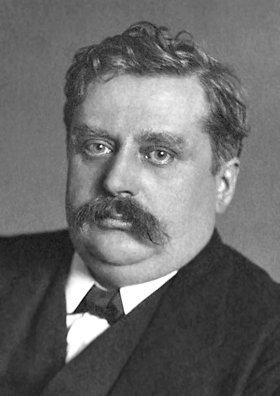
\includegraphics[width=\linewidth]{images/book3/werner.jpg}
\end{minipage}\hfill
\begin{minipage}[t]{0.74\linewidth}
\vspace{0pt}
اقترح ألفرد فرنر سنة 1893 أن للفلز، إلى جانب تكافئه،
عدد تناسق من المجموعات المثبتة حوله مباشرة، وأن الكوبالت(III) يحمل
ستًا منها عند رؤوس ثماني أوجه. ثم تنبأ بعدد المتماكبات التي ينبغي أن تكون لكل
صيغة وأمضى عشرين سنة في تحضيرها؛ وفي سنة 1911 فصل معقدًا
للكوبالت إلى متماكبيه المرآويين، مثبتًا أن الكيرالية لا تستلزم
ذرة كربون. ونال جائزة نوبل في الكيمياء سنة 1913. (صورة شخصية من الحولية «جوائز
نوبل»، 1914، ملكية عامة، ويكيميديا كومنز.)
\end{minipage}
\end{history}

\section{تمارين}

\begin{exercise}[$\star$]\label{exo:b2:coordination-complexes:1}
أعطِ توزيع $d^n$ للأيونات \ce{Ti^3+}، \ce{V^3+}، \ce{Cr^3+}، \ce{Mn^2+}، \ce{Fe^3+}،
\ce{Co^2+}، \ce{Ni^2+} و\ce{Zn^2+}.
\end{exercise}

\begin{exercise}[$\star$]\label{exo:b2:coordination-complexes:2}
أعطِ \omterm{def:b2:coordination-complexes:denticity}{عدد المخالب} للماء، وللإيثان-1،2-ثنائي الأمين، ولأيون الإيثانديوات، ولربيطة edta 
ولأيون الثيوسيانات، وقل أيها ثنائي الموقع.
\end{exercise}

\begin{exercise}[$\star$]\label{exo:b2:coordination-complexes:3}
سمِّ \ce{[Cu(NH3)4]SO4}، \ce{K3[Fe(CN)6]}، \ce{[CoCl2(NH3)4]Cl} 
و\ce{[Ni(CO)4]}.
\end{exercise}

\begin{exercise}[$\star$]\label{exo:b2:coordination-complexes:4}
تنبأ بهندسة \ce{[Ag(NH3)2]+}، \ce{[CoCl4]^2-}، \ce{[PtCl4]^2-} 
و\ce{[Fe(H2O)6]^2+}.
\end{exercise}

\begin{exercise}[$\star\star$]\label{exo:b2:coordination-complexes:5}
كم متماكبًا للمعقد المربع المستوي \ce{[PtCl2(NH3)2]}؟ ارسمها. (أحدها،
السيسبلاتين، دواء مضاد للسرطان.)
\end{exercise}

\begin{exercise}[$\star\star$]\label{exo:b2:coordination-complexes:6}
عُدّ إلكترونات التكافؤ في \ce{Cr(CO)6}، \ce{Fe(CO)5}، \ce{Ni(CO)4}،
\ce{V(CO)6} و\ce{Mn2(CO)10}. أيها يخالف القاعدة، وكيف يسلك؟
\end{exercise}

\begin{exercise}[$\star\star$]\label{exo:b2:coordination-complexes:7}
عُدّ إلكترونات التكافؤ في الفيروسين وفي الكوبالتوسين \ce{Co(C5H5)2}. أيهما
يتأكسد بسهولة، وإلى أي شيء؟
\end{exercise}

\begin{exercise}[$\star\star$]\label{exo:b2:coordination-complexes:8}
لمعقد النيكل(II) مع edta القيمة $\log_{10}K = 20.5$، وهي أعلى بكثير من قيم المعقدات التي
يرتبط فيها النيكل بست ذرات مانحة منفصلة من النيتروجين أو الأكسجين. فسّر هذا الأثر المخلبي
بعدد الجسيمات المحررة حين يحل المخلب محل ست جزيئات
ماء.
% ledger: logb:Ni-edta
\end{exercise}

\begin{exercise}[$\star\star$]\label{exo:b2:coordination-complexes:9}
ارسم \omterm{def:b2:coordination-complexes:isomers}{متماكبي الارتباط} للمعقد \ce{[Co(NO2)(NH3)5]^2+}.
\end{exercise}

\begin{exercise}[$\star\star\star$]\label{exo:b2:coordination-complexes:10}
كم متماكبًا فراغيًا للمعقد \ce{[CoCl2(en)2]+}؟ وأيها كيرالي؟
\end{exercise}

\begin{exercise}[$\star\star\star$]\label{exo:b2:coordination-complexes:11}
من أجل $\mathrm{MA_4B_2}$، عُدّ المتماكبات التي يتنبأ بها سداسي مستوٍ ومنشور
ثلاثي لست ربائط، وفسّر كيف يحسم عدد المتماكبات المكتشفة بين
الهندستين.
\end{exercise}

\begin{exercise}[$\star\star\star$]\label{exo:b2:coordination-complexes:12}
عُدّ إلكترونات التكافؤ في \ce{[RhCl(PPh3)3]} وفي \ce{[IrH(CO)(PPh3)3]}
(\ce{PPh3} مانح لإلكترونين، و\ce{H-} بوصفه هيدريدًا). أيهما يمكنه استقبال ربيطتين
إضافيتين؟
\end{exercise}

\section{مسألة: أمينات الكوبالت عند فرنر}

\begin{problem}[{مسألة نهاية الأسبوع --- أربعة أمينات لكلوريد الكوبالت(III) والكلوريد
الذي تحرره، وصيغها بالأقواس المعقوفة، ومتماكبا رباعي الأمين وما
يثبتانه عن الهندسة، والنشاط الضوئي لمعقد ثلاثي المخلب}]
\label{pb:b2:coordination-complexes:1}
المعطيات: أربعة مركبات، A \ce{CoCl3.6NH3} (برتقالي مصفر)، وB \ce{CoCl3.5NH3}
(أرجواني)، وC وD \ce{CoCl3.4NH3} (أخضر وبنفسجي). مع فائض من نترات الفضة،
يرسّب مول واحد من A ثلاثة مولات من \ce{AgCl}، وB مولين، وC وD مولًا واحدًا لكل منهما. 
وتُظهر الموصليات المولية 4 و3 و2 و2 أيونات لكل وحدة صيغة.

\medskip
\noindent\textbf{الجزء الأول --- الكلوريد والأيونات.}
\begin{enumerate}
  \item أي الكلوريدات تتفاعل فورًا مع أيونات الفضة؟
  \item كم كلوريدًا مرتبطًا بالكوبالت في كل مركب؟
  \item قارن أعداد الأيونات بالموصليات.
  \item ما عدد أكسدة الكوبالت في المركبات الأربعة؟
  \item ما توزيعه $d^n$؟
  \item ما العدد الكلي للربائط التي يحملها الكوبالت في كل مركب؟
\end{enumerate}

\medskip
\noindent\textbf{الجزء الثاني --- الصيغ والأسماء.}
\begin{enumerate}[resume]
  \item اكتب A وB وC وD بالأقواس المعقوفة.
  \item سمِّ A وB.
  \item سمِّ كاتيون C وD.
  \item ما نوع التماكب بين C وD؟
  \item ماذا يكون مركب \ce{CoCl3.3NH3}، وكم أيونًا يعطي؟
  \item كم متماكبًا يكون لذلك المركب في ثماني الأوجه؟
\end{enumerate}

\medskip
\noindent\textbf{الجزء الثالث --- الهندسة.}
\begin{enumerate}[resume]
  \item ارسم \ce{[CoCl2(NH3)4]+} في وضعي cis وtrans في ثماني الأوجه.
  \item عُدّ متماكبات \ce{[CoCl2(NH3)4]+} المتوقعة لست ربائط عند
        رؤوس سداسي مستوٍ.
  \item عُدّ المتماكبات المتوقعة لمنشور ثلاثي.
  \item لم يجد فرنر قط أكثر من اثنين. ماذا يثبت ذلك؟
  \item هل البرهان كامل؟ ماذا كان سيعني وجود متماكب ثالث؟
  \item أيّ المركبين C وD هو cis، علمًا أن المتماكب cis يمكن تحويله إلى
        معقد مخلبي مع الإيثانديوات بينما لا يمكن ذلك للمتماكب trans؟
\end{enumerate}

\medskip
\noindent\textbf{الجزء الرابع --- النشاط الضوئي.}
\begin{enumerate}[resume]
  \item ارسم \ce{[Co(en)3]^3+}.
  \item هل له مستوي مرآة؟ ومركز تناظر؟
  \item كم متماكبًا فراغيًا له؟
  \item ماذا يثبت فصل مثل هذا الكاتيون إلى متماكبين مرآويين؟
  \item هل \ce{[CoCl2(en)2]+} كيرالي في هيئته cis؟ وفي هيئته trans؟
  \item لماذا كان لفصل فرنر لمعقد لا يحوي أي كربون أهمية؟
  \item اذكر عدد متماكبات \ce{[CoCl2(NH3)4]+} التي يتنبأ بها ثماني الأوجه،
        وكلٌّ من السداسي المستوي والمنشور الثلاثي.
\end{enumerate}
\end{problem}
